% !TEX root = ./main.tex

\documentclass{article}
\usepackage[utf8]{inputenc}
\usepackage[ngerman]{babel}
\usepackage{pdfpages}
\usepackage{graphicx}
\usepackage{amsmath}

\graphicspath{ {./img/} }
\usepackage{hyperref}
\usepackage{lipsum}
\usepackage{float}
\usepackage{listings}

\usepackage{xcolor}

\definecolor{codegreen}{rgb}{0,0.6,0}
\definecolor{codegray}{rgb}{0.5,0.5,0.5}
\definecolor{codepurple}{rgb}{0.58,0,0.82}
\definecolor{backcolour}{rgb}{0.95,0.95,0.92}

\lstdefinestyle{mystyle}{
    backgroundcolor=\color{backcolour},   
    commentstyle=\color{codegreen},
    keywordstyle=\color{magenta},
    numberstyle=\tiny\color{codegray},
    stringstyle=\color{codepurple},
    basicstyle=\ttfamily\footnotesize,
    breakatwhitespace=false,         
    breaklines=true,                 
    captionpos=b,                    
    keepspaces=true,                 
    numbers=left,                    
    numbersep=5pt,                  
    showspaces=false,                
    showstringspaces=false,
    showtabs=false,                  
    tabsize=2
}

\lstset{style=mystyle}
\lstset{literate=%
{Ö}{{\"O}}1
{Ä}{{\"A}}1
{Ü}{{\"U}}1
{ß}{{\ss}}2
{ü}{{\"u}}1
{ä}{{\"a}}1
{ö}{{\"o}}1
}

\newcommand{\nr}{1}


\title{Aktorik Sensorik \\ Labor 2}
\author{Anton Kress (S872899), Jan Abel (S876662)}
\date{October 2020}

\begin{document}

\maketitle

\newpage
\tableofcontents 
\section{Einleitung und Ziel}

Im 4. Labor soll der zuvor modellierte, spannungsgesteuerte
Gleichstrommotor nun stromgesteuert werden. Dieses soll Mittels
eines Vierquadrantensteller auch H-Brücke genannt in Simulink
als Modell umgesetzt werden.



% \section{Einleitung und Ziel}

% Im 4. Labor im Modul Aktorik und Sensorik soll jubaefiubaefiu bestimmt werden.


% Was m"ussen Sie um das bestehende Motormodell hinzufügen, um einen Strom einprägen zu können?
% H-Br"ucke

% 2.1
% T_LH und T_RL

% 2.2 
% Durch die Drehung des Motors wird eine Spannung Induziert. Dadurch fließt ein Strom durch die 
% sogenannten Parasit"ardioden T_RH und T_LL. 

% 2.3
% Der Strom l"asst sich "uber R_shunt messen, welcher passenderweise mit 1 OHM gew"ahlt ist. So ist
% die Spannung, die an R_shunt abf"allt gleich des Stromes.

% 2.4
% Es gibt vier verschiedene Zust"ande. Wenn der Motor im Uhrzeigersinn betrieben werden soll, k"onnen
% die entsprechenden Transistoren geschaltet sein oder nicht geschaltet sein. Soll der Motor gegen
% den Uhrzeigersinn betrieben werden, kann das andere Transistorenpaar geschaltet sein oder nicht.

% 2.5
% Eing"ange: I_IST, I_Soll, U_H-Br"ucke
% Ausg"ange: U_Motor

% 2.6
% 1. Fall: AN
%     U_H = U_T_LH + U_Motor + U_T_RL + U_R_shunt

%     U_H = R_LH * I_m + (R_shunt * I_m)  

% 2. Fall: Aus
%     0 = U_H + U_D + U_Motor + U_D + U_shunt
%\include{laTex/as_labor04_04_grundlagen}
\subsection{Aufgabenstellung und Versuch}

Für das Subsystem Steuerung mit H-Brücke wurden folgenden Ein- und Ausgänge
definiert.\\

\begin{itemize}
    \item ($In_1$) Die Eingangs oder Betriebsspannung $U_H$
    \item ($In_2$) Der Momentanstrom $I_{ist}$
    \item ($In_3$) Der angestrebte Strom $I_{soll}$
    \item ($Out_1$) Die Spannung die über dem Motor abfällt $U_{Motor}$
\end{itemize}


\begin{figure}[H]
    \centering
    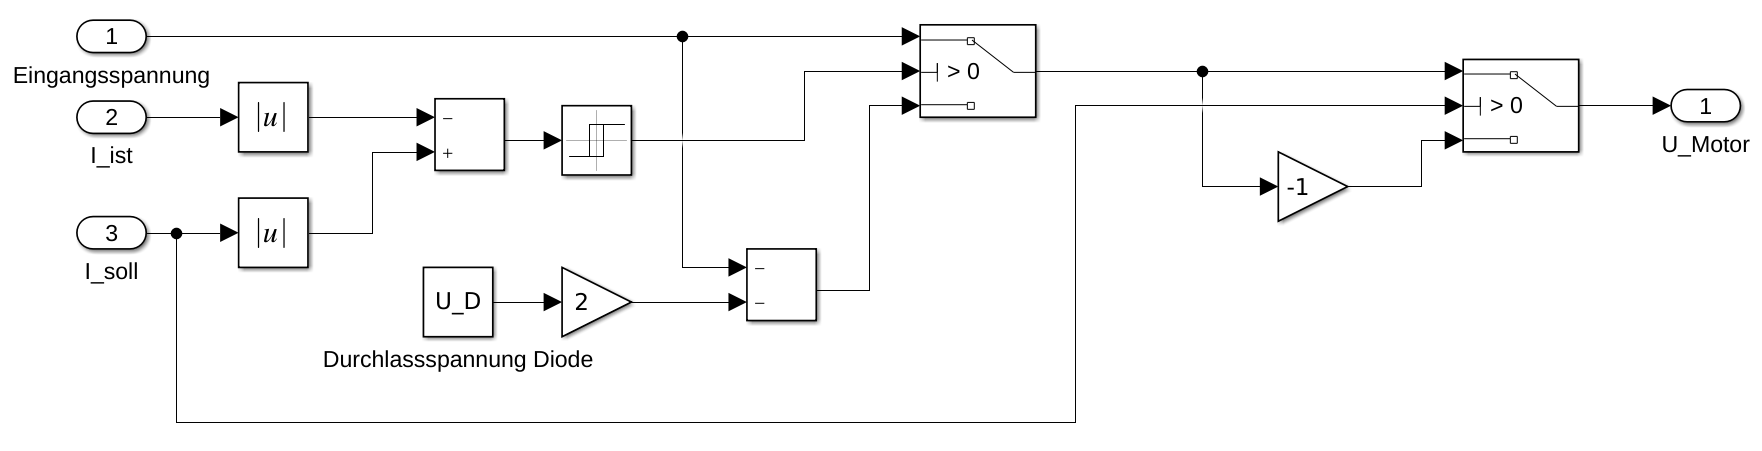
\includegraphics[width=1\textwidth]{hbridge_modell.png}
    \caption{Subsystem Steuerung mit H-Brücke}
    \label{fig:Subsystem H-Bridge}
\end{figure}

Das Subsystem beinhaltet Relay-Block der hier als Zweipunktregeler genutzt
wird. Die Beiden Schwellwerte $i_{plus}=10\mathrm{mA}$ und $i_{minus}=-10
\mathrm{mA}$ wurden im m-File definiert. Dieser gibt einen boolschen Wert
an den 1. Switch Block der zwischen Transistoren An und Aus hin- und
herschaltet. Der 2. Switch Block verändert die Drehrichtung des Motors und
wird geschaltet vom Vorzeichen des einzustellenden Strom $I_{soll}$.
\subsection{Zusammenfassung}

In diesem Versuch haben wir eine Steuerung mit H-Brücke modelliert und
sie mit dem Modell des Gleichstrommotor verbunden. Dieser lässt sich nun
Strom- statt Spannungs-gesteuert betreiben.
\section{Anhang}

\subsection{Aufgabenbeschreibung}
\begin{figure}[H]
    \centering
    \includegraphics[page=8, width=0.8\textwidth]{../Aufgabenstellung.pdf}
    %\caption{caption}
    \label{fig:Aufgabenstellung Labor 4.1}
\end{figure}

\begin{figure}[H]
    \centering
    \includegraphics[page=9, width=0.8\textwidth]{../Aufgabenstellung.pdf}
    \label{fig:Aufgabenstellung Labor 4.2}
\end{figure}

\subsection{Matlab Code}
\lstinputlisting[language=Matlab]{matlab/as_labor04_hbridge.m}

%\subsection{Messwerte}

\end{document}
